\documentclass[12pt,a4paper,titlepage,oneside,BCOR1cm]{scrreprt}



\usepackage[utf8]{inputenc}
\usepackage{graphicx}
\graphicspath{ {images/} } 
\usepackage[final]{pdfpages}
\usepackage{fancyhdr}
\usepackage[pagebackref,pdfpagelabels]{hyperref}
\usepackage{amsmath,amstext,amssymb}
\usepackage{rotating}
\usepackage{afterpage}

\bibliographystyle{gerunsrt} % Literaturangaben nach Auftreten sortieren %{gerplain}

\date{\today}
\author{Robin Maximilian Ruth}
\title{Bachelorthesis proposal -- Sparked}

\begin{document}
\thispagestyle{empty}

\begin{figure}[htbp]
\centering
 \begin{minipage}[b]{41 mm}
   
\includegraphics[width=40 mm]{./figures/DAI_Logo.png}
 \end{minipage}
\end{figure}

~\vspace{0.5cm}

\begin{center}
\begin{Huge}
Technische Universitaet Berlin\\
\vspace{1mm}
\end{Huge}{\Large Fakultaet IV - Elektrotechnik und Informatik\\
Fachgebiet AOT\\
Prof. Dr. Sahin Albayrak}\\

\vspace{26mm}
\begin{LARGE}
Bachelorthesis proposal\\
\end{LARGE}
\vspace{8mm}
\begin{LARGE}
Sparked, an intuitive user interface for the automated machine learning project CODA\\
\end{LARGE}
\vspace{3 cm}
Robin Ruth\\
Matrikel--Nummer 316672\\
\vspace{1cm}
\begin{tabular}{lll}
    \textbf{Betreuer} & Researcher Christian Geissler & Dipl.-Inform. ABC\\
\end{tabular}

\end{center}

\tableofcontents
\thispagestyle{empty}
%\addcontentsline{toc}{chapter}{Inhaltsverzeichnis} 


\pagenumbering{arabic}
\chapter{Motivation}
From gaming AIs to automated driving, from credit card fraud to spam detection, machine learning has already gained a significant place in todays society. 
These developments came over the last decades and are predicted to rise in usage and usability in the coming years.
All in all, machine learning is gearing up to be one of the dominant technologies of the 21st century. 

On a grand scale machine learning has the possibility to take huge amounts of work off of our shoulders. 
But even though the name might imply and some journalists may have writen as if one could just give a problem to an AI and wait for the solution, the reality in machine learning is not quite that simple.
Solving problems with machine learning, with best possible result for the relevant metric, having them train enough without being overfitted and have good properties in respect to runtime and resource usage, is still very much dependent on selecting the right tool for the right job and that is still primarily done by rare specialists. 
Therefor even though it is called machine learning, a human still selects the best classification method and configures it with a good set of hyperparameters and a human must evaluate the results of the learning phase with a metric they think is appropriate.
This process is unfortuatelly very timeconsuming and does not guaranty the best results.

With the project CODA GT-ARC is doing fundamental research in automated machine learning and hyperparameteroptimisation, to allow the CODA to make these selections for the user. 
Reducing the guesswork and need for human action in the creation of machine learning solutions could elevat the field of machine learning to a new level, where the atvantages could be used much more widespread and the experts could use their talents in a more productive manner.

Sparked builds on top of that, trying to give machine learning specialists and enthusiasts a clear and easy to use interface to interact with the current and future versions of the CODA project. 
Selecting out of the growing number of evaluation methods, metrics and test data, to pick a classifier and select its hyperparameters or request CODA to find the best parameters automatically and display the results in a visually appealing way, Sparked tries to streamline this process, for the user to easily create and compare testruns with selections of classifiers and hyperparameters or evaluate the automatical selected done by CODA.

\chapter{Objective}
The objective of Sparked is to create a web program to create orders out of a given amount of parameterised classifiers, evaluation methods, metrics and testdata, to have them evaluated by CODA and to display the results in a helpful manner.

The configuration values (parameterised classifier, evaluation mehtod, metric and testdata) will be supplied dynamically by CODA, to allow CODA to grow in its possibilities without needing to rebuild this program.
From an order a set of tasks will be generated, that will successively be send to CODA for evaluation.
If an order has been finished, it should be possible to view its result. 

The user interface of Sparked has three main goals. 
\begin{itemize}
\item Make the handling of Sparked self-explanatory enough for machine learning experts to use it without the need of prior training. 
\item Show the results in a way to allow the user to draw the needed conclusions.
\item Create a user interface that is visually appealing enough to be used in demonstrations.
\end{itemize}

While the last point will be at the viewers disgression, the first two points will be evaluated by allowing an expert a limited time of use of the final program and interviewing them on their opinion on the handling and helpfullness in the evaluation of an order.
Because of timeconstraints it will not be part of this thesis to make a full quantitativ analysis, but to make a qualitativ analysis instead.

Naturally Sparked will have to compare to existing programs with a similar objective. 
While we will not compare the results as given by the CODA backend with those of other projects, comparing the selected ways to present them is part of this thesis.

\chapter{Work packages}

\begin{itemize}
\item Evaluating technologies

\item Technical setup
\begin {itemize}
\item get everything running on docker
\item link docker images
\item move git repo to the gt-arc repo
\item ensure that everything runs on the dai labor linux VMs
\end{itemize}
\item Evaluation state of the art
\begin{itemize}
\item Find accessible similar programs
\item Find programs that have to solve similar ui issues
\begin{itemize}
\item Diplay graphs
\item Display complex lists with subelements
\item Select values and set their parameters from a list
\end{itemize}
\end{itemize}

\item Research
\begin{itemize}
\item Generic research in the fields of hyperparameter optimization and automated machine learning
\item Specific research: What does the user of spark need to see to make evaluate order results
\end{itemize}

\item Programming
\begin{itemize}
\item Creating controllers
\item Saving and loading data from database
\item Access CODA REST endpoint for configuration and evaluation interface
\item Access data in frontend

\item Create UI functionality
\begin{itemize}
\item List orders
\item Create order
\item Display results
\end{itemize}
\end{itemize}
\item Bugfixing
\item Evaluation of usability 
\begin{itemize}
\item Preparing interview
\begin{itemize}
\item Create questionair
\item Find suitable person
\end{itemize}
\item Conduct interview
\item Evaluate interview
\end{itemize}

\item Writing thesis
\begin{itemize}
\item Feedback and corrections
\end{itemize}
\item Presentation
\end{itemize}

\section{UI functionality}
In this section we will define the needed functionality. 
These functionality blocks may, but do not have to belong to concrete views in the finished program. 
How they are grouped, displayed and designed is part of the work of this thesis.
Since programming will take quite a bit of the available time, the functionality in here should be complete. 
Adding functionality afterwards should not happen, to keep the scope of the project managable.

\subsection{List orders}
This allows the user to view all orders in the system, regardless of whom created them. 
It will show their status (waiting, paused, running, finished, error) and allows them under specific circumstances to be paused, continued or opened to show the results.
Since an order is a set of tasks, there needs to be a way to view the list of tasks an order is comprised of. 
There we want to give the user feedback on wich task is running and the evaluation status as given by the CODA backend. 

\subsection{Create order}
The user wants to create a new order. 
To create an order they need to be able to select classifiers with available parameters, the validation method with available parameters, the metric which this is evaluated against and the dataset that is used.
These configuration parameters will be dynamically loaded from a REST endpoint from the CODA server. 
They can not be edited from Sparked.
An instance of Sparked should for its whole life time only be connected to the same CODA instance. 

If an order has been defined, it will be split in tasks, saved and can then be viewed (See list orders functionality)

\subsection{Display results}
If an order is finished, Sparked gives the opportunity to view the results. 
Displaying these results should help the user to draw the conclusions they need. 
Identifing the questions a user might want answered is part of this thesis.

\section{Programming}
To facilitate the needed frontend functionality, a backend will be developed. 
This will at least contain a way to persist data and to access the CODA endpoint.

\chapter{Schedule}
The Gantt diagram shows the known work packages with their dependencies. See Appendix for larger version.

\hspace*{-1.5in}
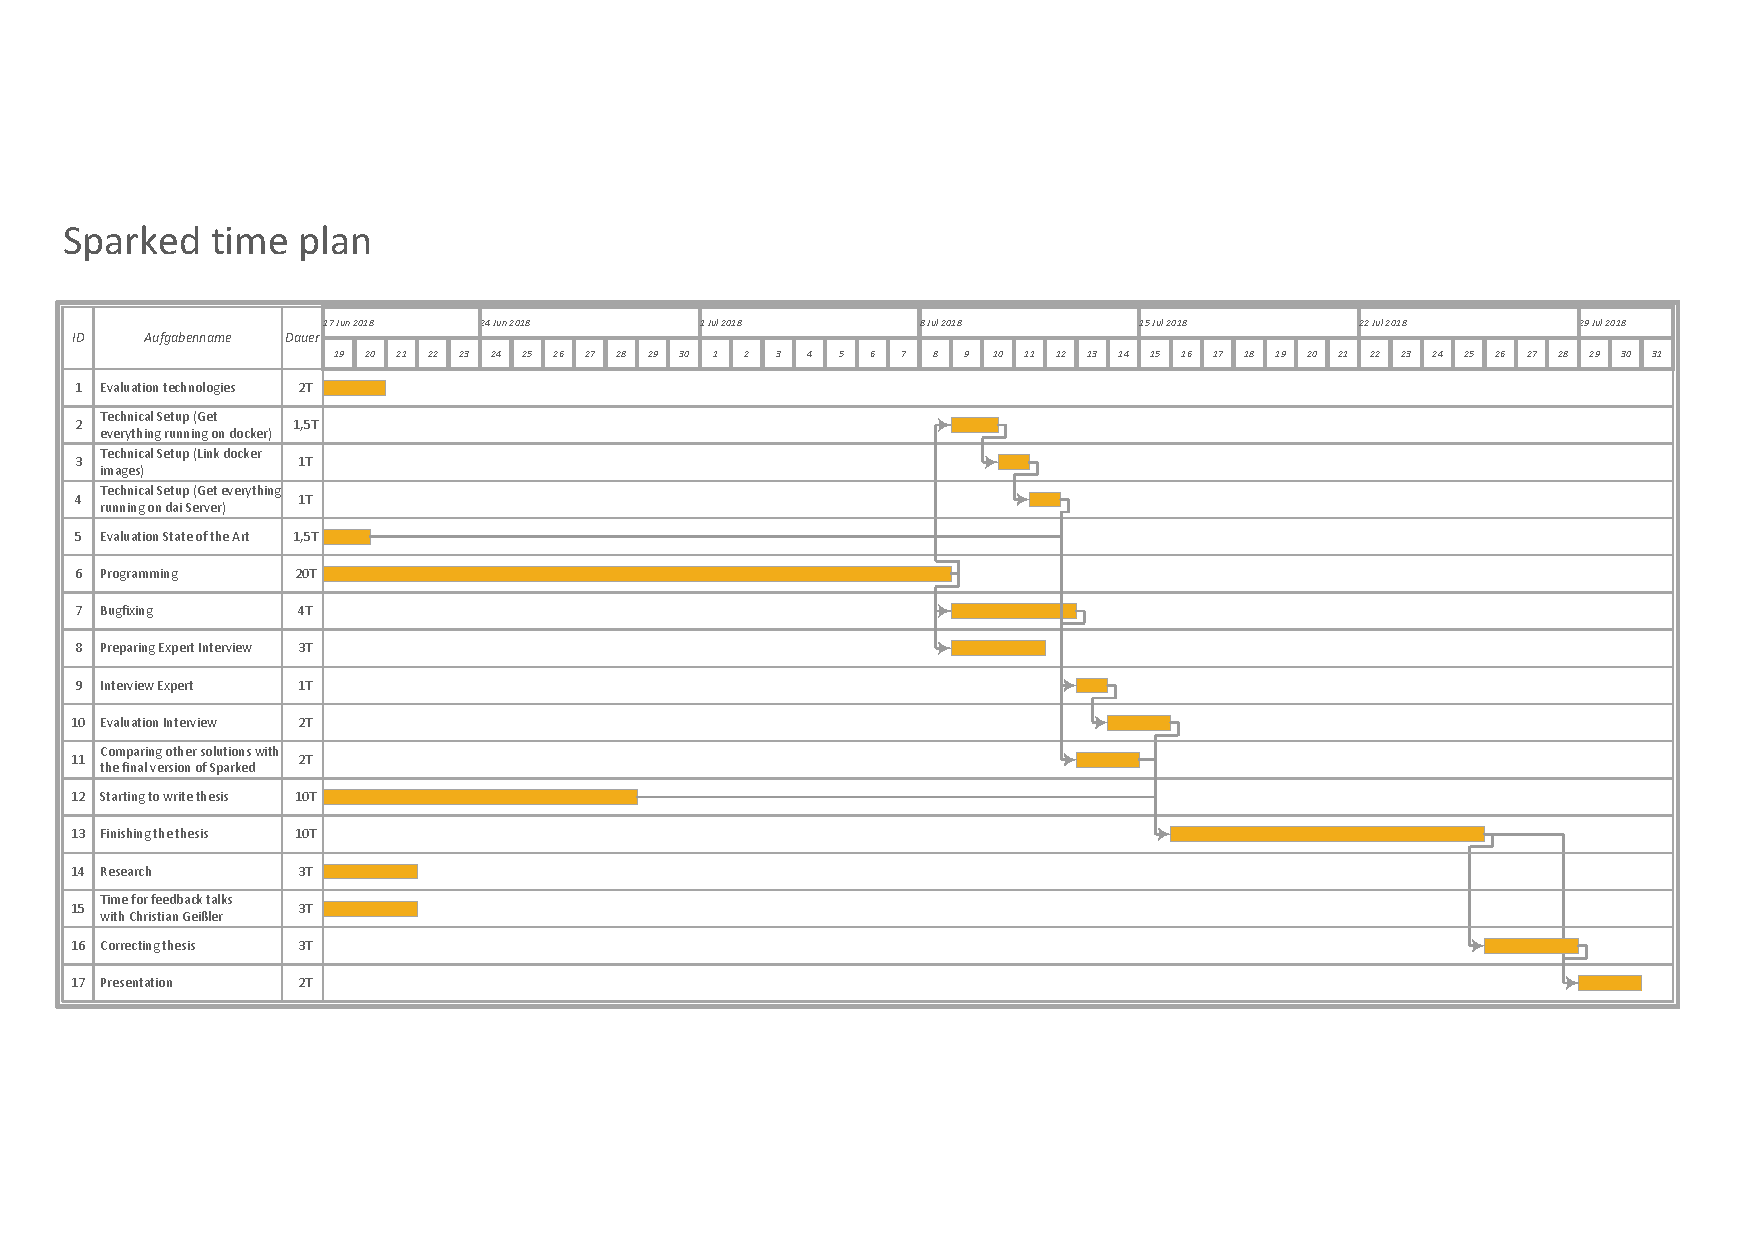
\includegraphics[width=\paperwidth]{gantt-proposal.pdf}

\chapter{Organizational}
\begin{itemize}
\item Language of this Bachelorthesis is english.
\item The thesis will be written with pdflatex.
\item Choosing programming languages and technologies are not defined and part of the development process.
\item Supervisors is Christian Geißler
\item Evaluators are Prof. Dr. Albayrak and Prof. Kao
\end{itemize}

\chapter{Appendix}

\afterpage{
\thispagestyle{empty}
\vspace*{-1.2in}
\hspace*{-1.5in}
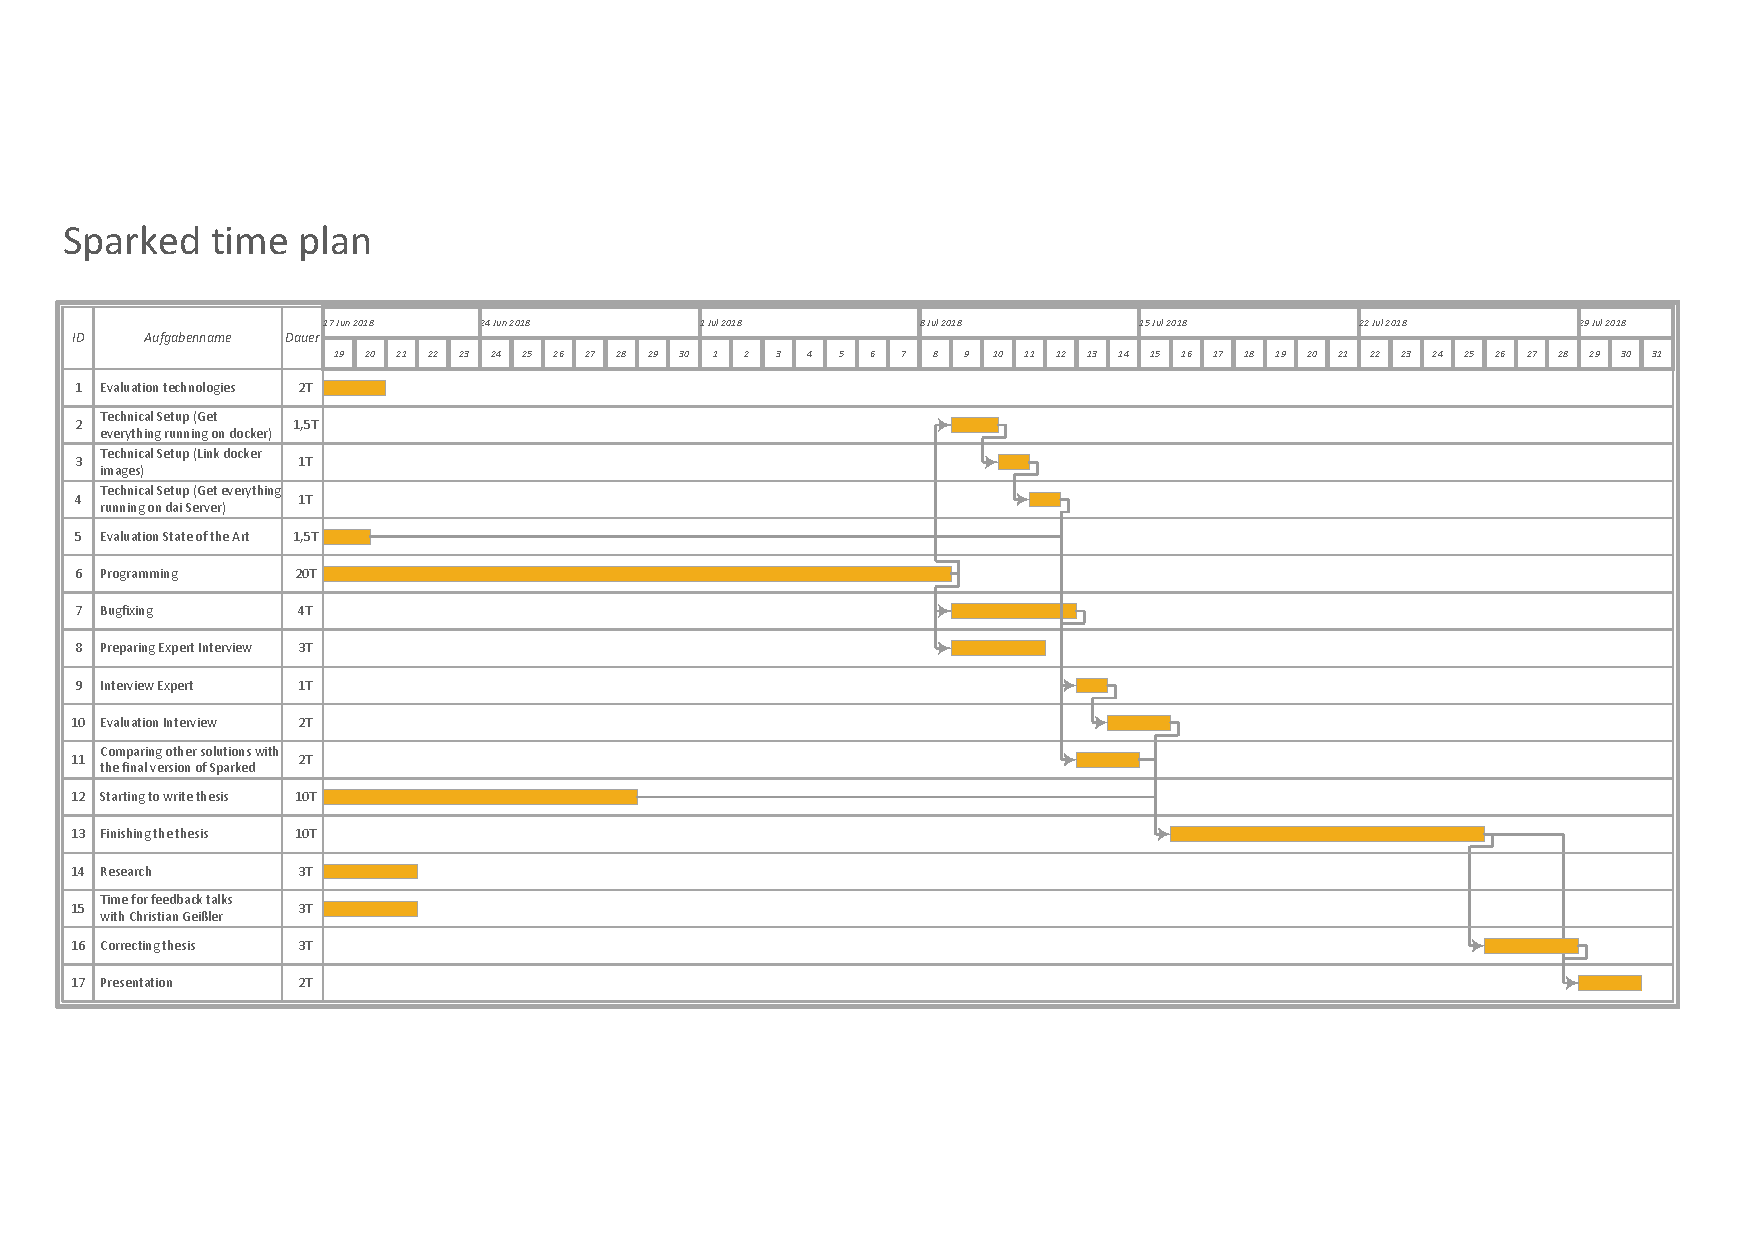
\includegraphics[angle=90, height=\paperheight]{gantt-proposal.pdf}
}
\newpage

\nocite{*}
\bibliography{chapter/bibliography} % Literaturverzeichnis
\addcontentsline{toc}{chapter}{Literaturverzeichnis}

\end{document}
